% =====================================================================
% StudyVault — Cumplimiento de la Rúbrica
% Compilar con: pdflatex cumplimiento.tex  (o subir a Overleaf)
% =====================================================================
\documentclass[11pt,a4paper]{article}

% ---------- Preámbulo ----------
\usepackage[utf8]{inputenc}
\usepackage[T1]{fontenc}
\usepackage[spanish,es-tabla]{babel}
\usepackage{lmodern}
\usepackage{amssymb}
\usepackage[margin=2.2cm]{geometry}
\usepackage{xcolor}
\usepackage{hyperref}
\usepackage{graphicx}
\usepackage{longtable}
\usepackage{booktabs}
\usepackage{array}
\usepackage{enumitem}
\usepackage{fancyhdr}
\usepackage{titlesec}
\usepackage{listings}
\usepackage{tcolorbox}
\usepackage{caption}
\usepackage{float}

\graphicspath{{capturas/}}

\definecolor{svprimary}{HTML}{4F46E5}
\definecolor{svaccent}{HTML}{F59E0B}
\definecolor{svsuccess}{HTML}{16A34A}
\definecolor{svdanger}{HTML}{DC2626}
\definecolor{svbg}{HTML}{F8FAFC}

\hypersetup{
    colorlinks=true,
    linkcolor=svprimary,
    urlcolor=svprimary,
    pdftitle={StudyVault - Cumplimiento de la Rubrica},
    pdfauthor={Jose Roberto Garcia Correa}
}

\pagestyle{fancy}
\fancyhf{}
\fancyhead[L]{\textbf{StudyVault}}
\fancyhead[R]{Cumplimiento de la Rúbrica}
\fancyfoot[C]{\thepage}

\titleformat{\section}{\Large\bfseries\color{svprimary}}{\thesection.}{0.5em}{}
\titleformat{\subsection}{\large\bfseries\color{svprimary!85}}{\thesubsection}{0.5em}{}

\lstset{
    basicstyle=\ttfamily\footnotesize,
    breaklines=true,
    frame=single,
    backgroundcolor=\color{svbg},
    keywordstyle=\color{svprimary},
    commentstyle=\color{gray},
    showstringspaces=false
}

\newcommand{\cumple}{{\color{svsuccess}\textbf{\large \checkmark{} Cumple}}}
\newcommand{\parcial}{{\color{svaccent}\textbf{\large $\bullet$ Parcial}}}
\newcommand{\nocumple}{{\color{svdanger}\textbf{\large $\times$ No cumple}}}

\newtcolorbox{evidencia}{
    colback=svbg,
    colframe=svprimary,
    sharp corners,
    boxrule=0.5pt,
    fonttitle=\bfseries,
    title=Evidencia
}

% =====================================================================
\begin{document}

\begin{titlepage}
\centering
\vspace*{2cm}
{\Huge\bfseries\color{svprimary} StudyVault\par}
\vspace{0.5cm}
{\Large Gestor de material de estudio con repetición espaciada\par}
\vspace{2.5cm}
{\LARGE\bfseries Cumplimiento de la Rúbrica\par}
\vspace{0.3cm}
{\large Análisis punto por punto frente a \texttt{descripcion.md}\par}
\vspace{3cm}

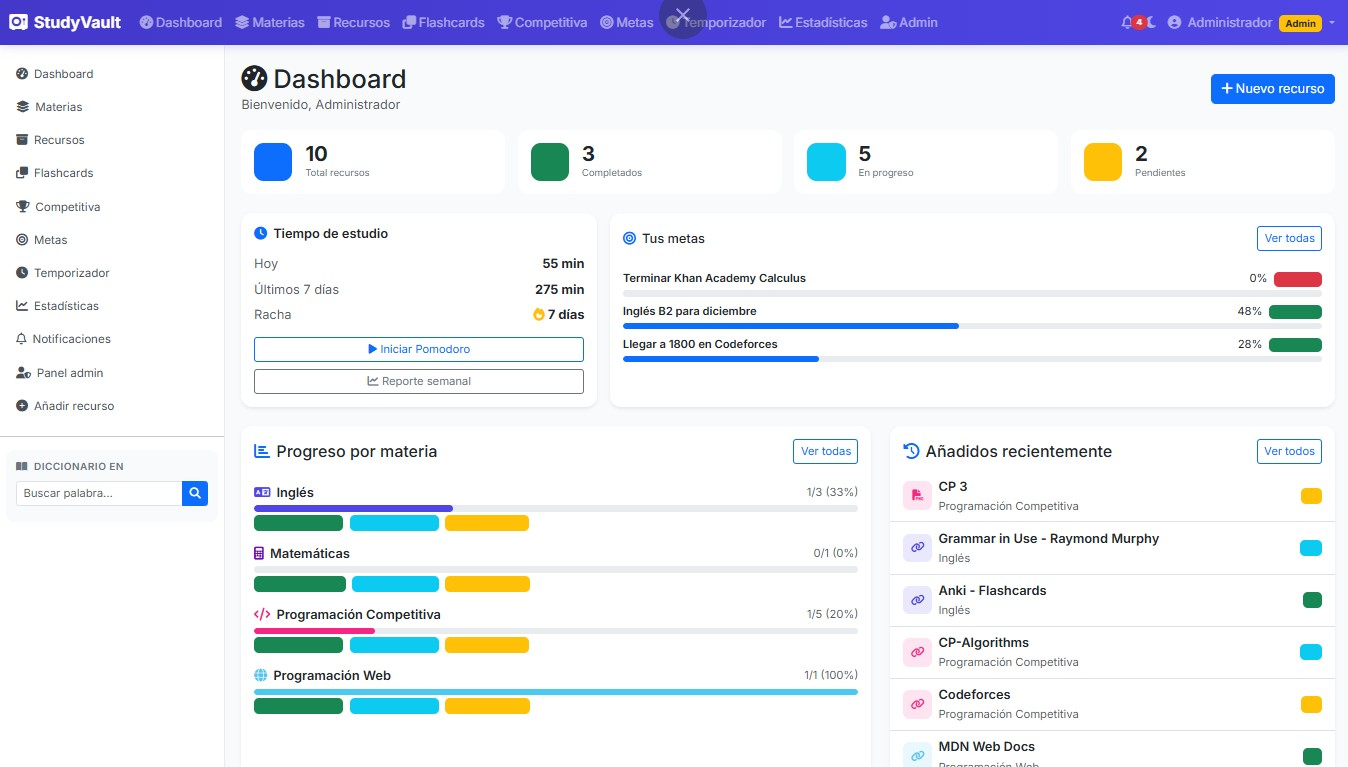
\includegraphics[width=0.85\linewidth]{cap_01_dashboard.jpg}
\vspace{1cm}

\begin{tabular}{ll}
\textbf{Autor:}      & José Roberto García Correa \\
\textbf{Materia:}    & Programación Web \\
\textbf{Semestre:}   & Sexto \\
\textbf{Fecha:}      & Mayo 2026 \\
\textbf{Repositorio:} & StudyVault (rama \texttt{develop}) \\
\end{tabular}

\vfill
\end{titlepage}

% ---------------------------------------------------------------------
\section{Tabla resumen}
\textbf{Leyenda:} \cumple{} \quad \parcial{} \quad \nocumple{}

\vspace{0.3cm}

\begin{longtable}{p{0.7cm} p{8cm} p{5cm}}
\toprule
\textbf{\#} & \textbf{Requisito} & \textbf{Estado} \\
\midrule
\endhead

Gen & Especificaciones generales (8 puntos) & \cumple \\
1 & Interfaz Web (HTML + CSS) & \cumple \\
2 & Cliente (JavaScript) & \cumple \\
3 & Servidor (PHP OOP) & \cumple \\
4 & Base de datos MySQL & \cumple \\
5 & Autenticación, sesiones y \textbf{roles} & \cumple \newline {\small (Invitado + Admin)} \\
6 & Funcionalidades dinámicas obligatorias & \cumple \newline {\small (DataTables + Admin)} \\
7 & AJAX / fetch & \cumple \\
8 & Consumo de servicios web (4 APIs) & \cumple \\
9 & Seguridad mínima & \cumple \newline {\small (supera lo pedido)} \\
10 & Arquitectura MVC & \cumple \\
\midrule
Opc & Tema oscuro & \cumple \\
Opc & Bitácora de acciones & \cumple \\
Opc & Recuperación de contraseña & \cumple \\
Opc & Exportar PDF o Excel & \cumple \newline {\small (CSV + PDF)} \\
Opc & Gráficas estadísticas & \cumple \newline {\small (6 Chart.js)} \\
Opc & Notificaciones & \cumple \\
Opc & Panel administrativo & \parcial \newline {\small (mini-panel)} \\
\bottomrule
\end{longtable}

\textbf{Conclusión:} 10 de 10 requisitos obligatorios cumplidos, 6 de 7 mejoras opcionales implementadas, 1 parcial. Sin requisitos no cumplidos.

\newpage

% ---------------------------------------------------------------------
\section{Especificaciones generales}

Las 8 especificaciones generales de \texttt{descripcion.md} están cubiertas:

\begin{itemize}[leftmargin=*]
    \item \textbf{HTML5 / CSS3} -- Bootstrap 5 + \texttt{assets/css/app.css} (custom).
    \item \textbf{JavaScript y AJAX/fetch} -- \texttt{assets/js/app.js} + scripts por vista.
    \item \textbf{PHP orientado a objetos} -- \texttt{models/}, \texttt{controllers/}, autoload con \texttt{spl\_autoload\_register}.
    \item \textbf{PDO con consultas preparadas} -- \texttt{config/database.php} + todos los modelos.
    \item \textbf{MySQL} -- 16 tablas relacionales.
    \item \textbf{Sesiones y seguridad} -- sesión segura, CSRF, hashing bcrypt, throttling, cabeceras (CSP).
    \item \textbf{Consumo de servicios web} -- 4 APIs públicas integradas vía proxy PHP.
    \item \textbf{Diseño responsivo} -- Bootstrap responsive + modo oscuro.
\end{itemize}

% ---------------------------------------------------------------------
\section{Requisitos mínimos (10 puntos)}

\subsection{Interfaz Web -- \cumple}
Responsive, navbar + sidebar, formularios estructurados, CSS externo (\texttt{app.css}), tablas estilizadas, componentes modernos. Bootstrap y Font Awesome incluidos. DataTables aprovechado para ordenamiento por columna.

\begin{figure}[H]\centering
    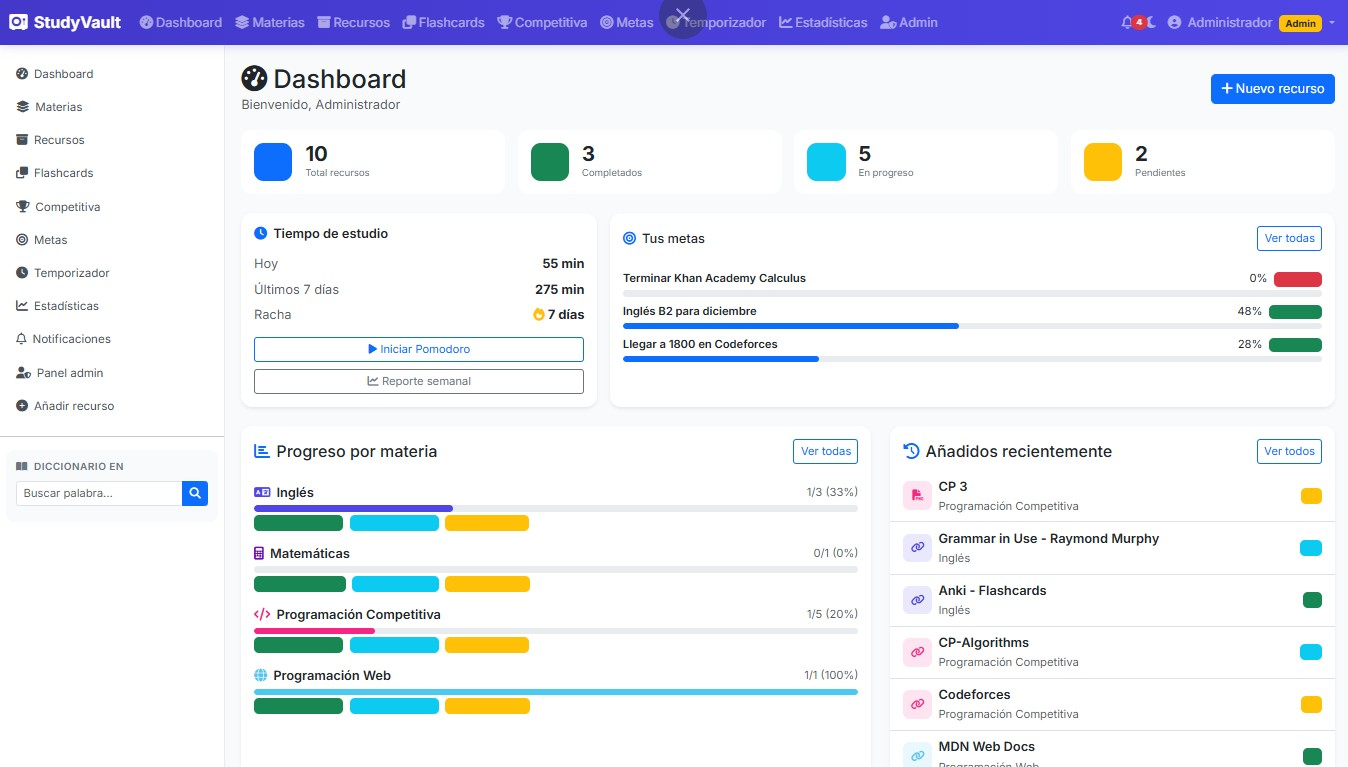
\includegraphics[width=0.95\linewidth]{cap_01_dashboard.jpg}
    \caption{Dashboard administrativo con tarjetas de stats, tiempo de estudio, racha y metas.}
\end{figure}

\subsection{Cliente (JavaScript) -- \cumple}
Validaciones dinámicas (formularios, coincidencia de contraseñas), eventos, manipulación del DOM, fetch, actualización parcial sin recargar, búsquedas y filtros instantáneos (Recursos), alertas dinámicas, modo oscuro persistente.

\subsection{Servidor (PHP OOP) -- \cumple}
MVC con clases y métodos, \textbf{inclusión modular} (\texttt{config/init.php} + autoloader), \textbf{reutilización} (motor SM-2 compartido entre flashcards y CP). CRUDs completos (materias, recursos, unidades, metas, flashcards, problemas CP, plantillas). Validación en servidor, manejo de errores centralizado (\texttt{set\_exception\_handler} + log), sanitización (\texttt{htmlspecialchars} + preparadas).

\subsection{Base de datos MySQL -- \cumple}
Modelo relacional (16 tablas), PK/FK, relaciones 1:N y N:M (\texttt{goal\_resources}), integridad referencial (\texttt{ON DELETE CASCADE}), índices. PDO + consultas preparadas obligatorias.

\subsection{Autenticación, sesiones y roles -- \cumple}
Login, logout, sesiones, roles \texttt{admin}/\texttt{student}, \texttt{password\_hash}/\texttt{password\_verify}, protección de rutas (\texttt{requireLogin}/\texttt{requireAdmin}). Supera el mínimo con CSRF, throttling y regeneración de sesión.

\textbf{Roles diferenciados:}
\begin{itemize}[leftmargin=*]
    \item \textbf{Admin:} accede al mini-panel administrativo (gestión de usuarios + uso global).
    \item \textbf{Student:} usuario regular.
    \item \textbf{Invitado:} sin sesión, puede explorar plantillas públicas en modo solo lectura.
\end{itemize}

\begin{figure}[H]\centering
    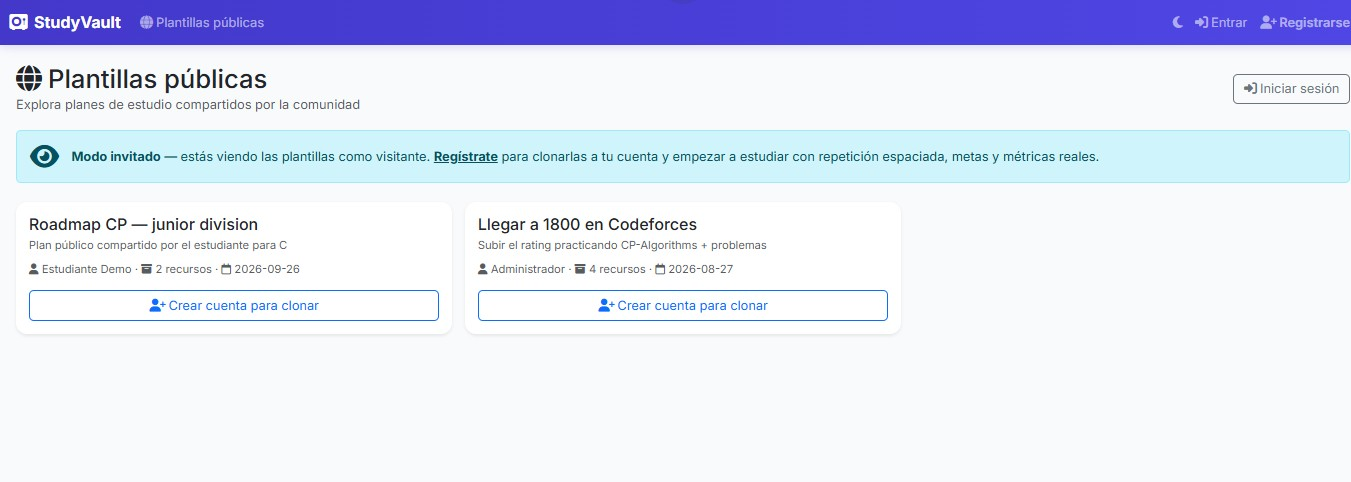
\includegraphics[width=0.85\linewidth]{cap_07_invitado.jpg}
    \caption{Rol \textbf{Invitado}: el navbar se simplifica, sin acceso a las funciones privadas. Sólo puede explorar plantillas públicas y registrarse para clonarlas.}
\end{figure}

\subsection{Funcionalidades dinámicas obligatorias -- \cumple}
Paginación, búsquedas, filtros, CRUD, subida de archivos (PDF/imágenes, máx. 50 MB), dashboard, \textbf{ordenamiento por columna} con DataTables en Recursos / Flashcards / Competitiva / Admin, y panel administrativo con activar/desactivar usuarios.

\begin{figure}[H]\centering
    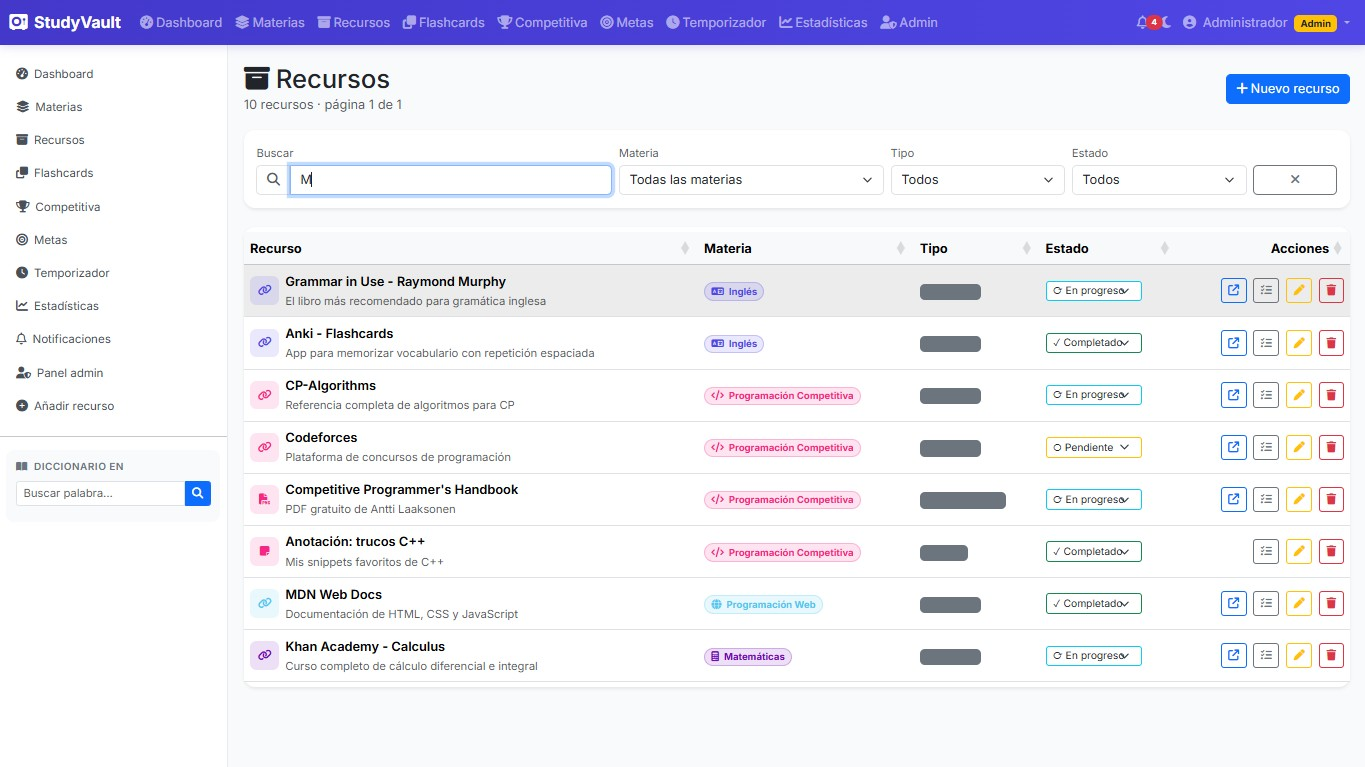
\includegraphics[width=0.95\linewidth]{cap_02_recursos.jpg}
    \caption{Listado de Recursos con búsqueda en vivo, filtros por materia/tipo/estado, paginación server-side y ordenamiento por columna.}
\end{figure}

\begin{figure}[H]\centering
    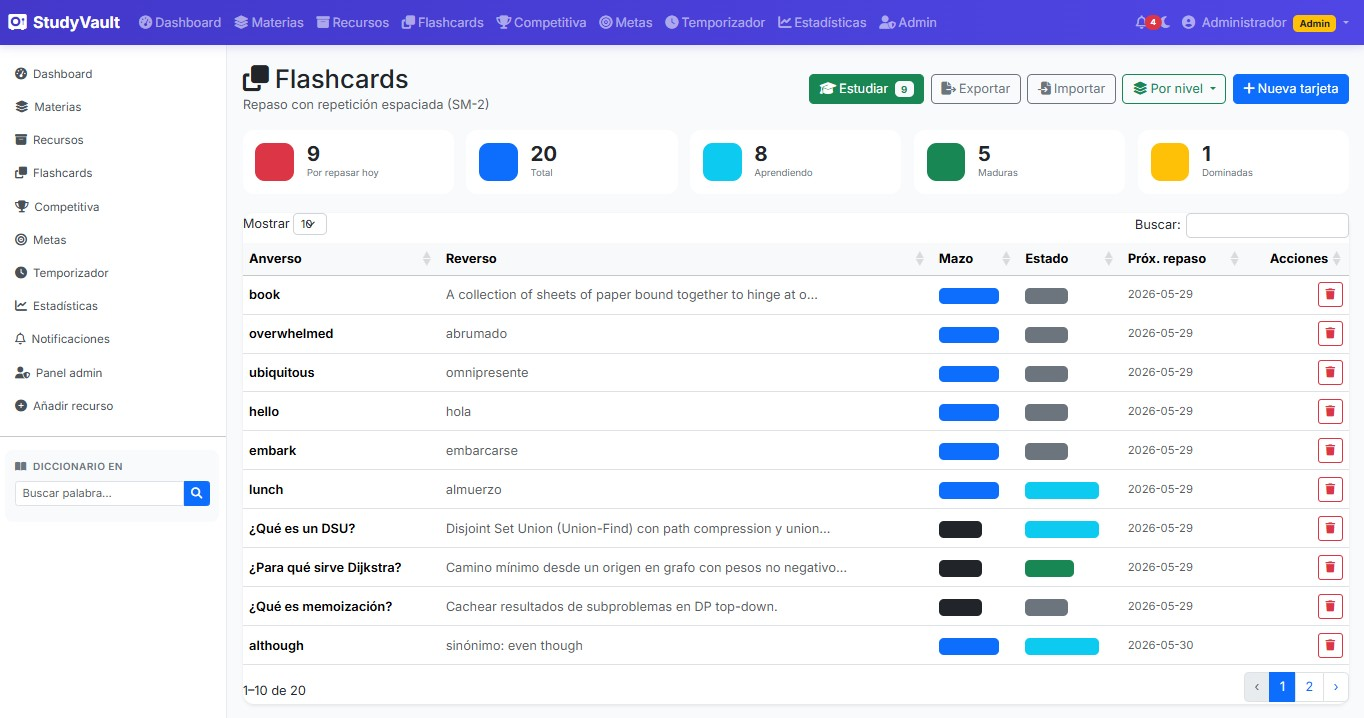
\includegraphics[width=0.95\linewidth]{cap_03_flashcards_tabla.jpg}
    \caption{Tabla de Flashcards con DataTables activo (encabezados ordenables) y tarjetas de estadísticas por estado SM-2.}
\end{figure}

\subsection{AJAX / fetch -- \cumple}
Consultas automáticas, actualización de tablas (búsqueda en vivo de Recursos), eliminación sin recargar, formularios dinámicos (modales), búsqueda en tiempo real, diccionario, repaso de flashcards / CP, centro de notificaciones, panel admin. Uso extenso.

\subsection{Consumo de servicios web -- \cumple{} (supera el mínimo)}
4 APIs públicas gratuitas, sin API key:

\begin{table}[H]\centering
\begin{tabular}{lll}
\toprule
\textbf{API} & \textbf{Uso} & \textbf{Endpoint} \\
\midrule
Free Dictionary & Definición, fonética, audio & \texttt{dictionaryapi.dev} \\
Datamuse & Colocaciones (uso real) & \texttt{api.datamuse.com} \\
Tatoeba & Frases de ejemplo reales & \texttt{tatoeba.org} \\
Codeforces & Rating, problemas, concursos & \texttt{codeforces.com/api} \\
\bottomrule
\end{tabular}
\end{table}

Todas se consumen vía proxy PHP (evita CORS + caché + rate limiting).

\begin{figure}[H]\centering
    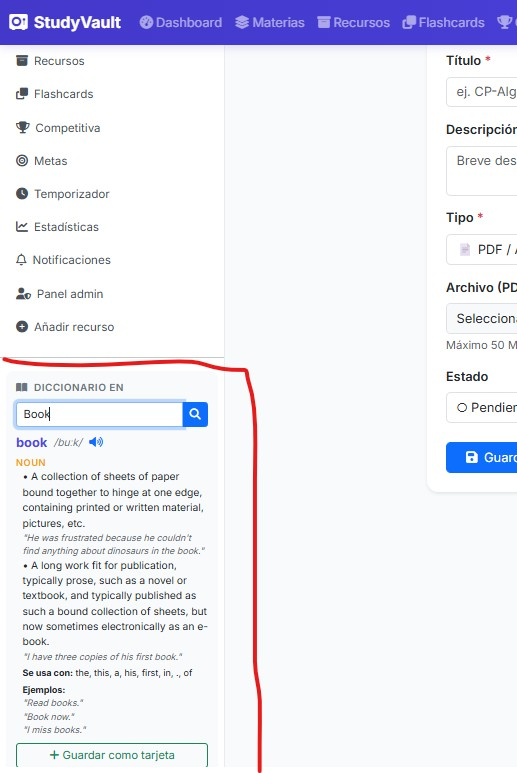
\includegraphics[width=0.65\linewidth]{cap_04_diccionario.jpg}
    \caption{Diccionario integrado en la barra lateral: definición (Free Dictionary) + ``se usa con'' (Datamuse) + frases de ejemplo (Tatoeba), con botón ``Guardar como tarjeta''.}
\end{figure}

\begin{figure}[H]\centering
    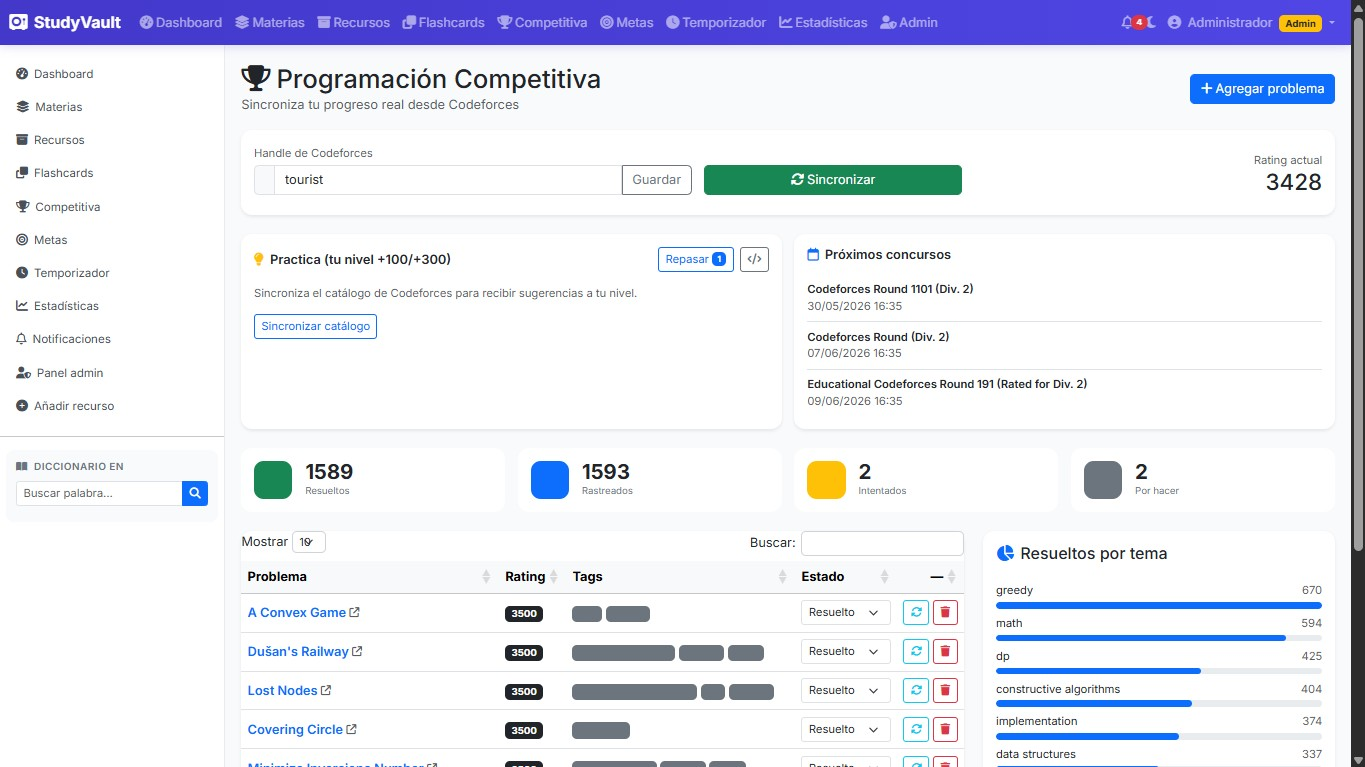
\includegraphics[width=0.95\linewidth]{cap_05_competitiva.jpg}
    \caption{Panel de Programación Competitiva: handle de Codeforces sincronizado, rating, problemas importados, análisis por tag y sugerencias de práctica.}
\end{figure}

\subsection{Seguridad mínima -- \cumple{} (supera lo pedido)}
\begin{itemize}[leftmargin=*]
    \item \textbf{Validaciones cliente/servidor:} en cada formulario.
    \item \textbf{Anti SQL Injection:} PDO preparado en TODAS las queries.
    \item \textbf{Anti IDOR:} cada query filtra por \texttt{user\_id} -- tests automatizados en \texttt{tests/security\_test.php}.
    \item \textbf{Sanitización:} \texttt{htmlspecialchars()} en salidas.
    \item \textbf{Extras:} CSRF en todo POST, \texttt{password\_hash} (bcrypt), \texttt{session\_regenerate\_id}, cabeceras (\texttt{X-Frame-Options}, \texttt{nosniff}, \texttt{Referrer-Policy}, \textbf{CSP}), rate limiting, throttling de login, \texttt{.htaccess} que bloquea ejecución en \texttt{uploads/}.
\end{itemize}

\subsection{Arquitectura MVC -- \cumple}
\texttt{config/}, \texttt{models/}, \texttt{controllers/}, \texttt{views/}, \texttt{assets/}\{css,js,img\} + \texttt{api/} para los endpoints AJAX. Coincide con la estructura recomendada.

\begin{lstlisting}[caption=Estructura de carpetas]
studyvault/
  config/       init.php  database.php  config.php
  models/       User, Resource, Subject, Flashcard, CpProblem, Goal, ...
  controllers/  AuthController, ResourceController, StatsController, ...
  views/        auth/  dashboard/  flashcards/  cp/  goals/  admin/  ...
  api/          dictionary.php  datamuse.php  tatoeba.php  search.php  ...
  assets/       css/  js/  vendor/  uploads/
  tests/        sm2_test.php  goal_test.php  security_test.php  ...
\end{lstlisting}

\newpage

% ---------------------------------------------------------------------
\section{Funcionalidades opcionales (mayor calificación)}

\subsection{Nivel intermedio}

\subsubsection{Recuperación de contraseña -- \cumple}
Flujo con token: tabla \texttt{password\_resets} (token de 32 bytes hex, expiración 1h, marca \texttt{used} al canjearse). Como XAMPP no tiene SMTP, el enlace se muestra en pantalla en modo demo.

\begin{figure}[H]\centering
    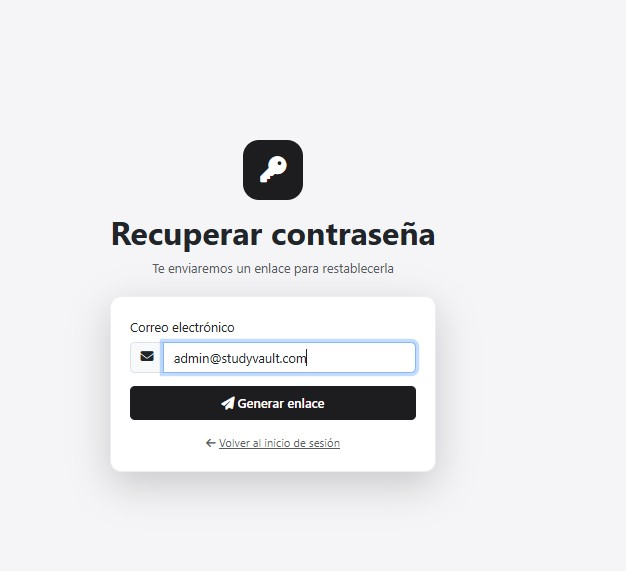
\includegraphics[width=0.6\linewidth]{cap_10_recuperar.jpg}
    \caption{Formulario ``Recuperar contraseña'' al que se accede desde el login.}
\end{figure}

\subsubsection{Exportar PDF o Excel -- \cumple}
\textbf{CSV} de flashcards compatible con Anki, \textbf{PDF} del reporte semanal y de las metas vía \texttt{window.print()} + CSS \texttt{@media print} (sin dependencias).

\subsubsection{Gráficas estadísticas -- \cumple}
Chart.js (servido localmente desde \texttt{assets/vendor/}), 6 gráficas en \texttt{?page=stats}:
\begin{enumerate}[leftmargin=*]
    \item Minutos de estudio por día (barras, 30 días).
    \item Tarjetas por estado SM-2 (doughnut).
    \item Vocabulario por nivel CEFR (barras horizontales).
    \item Problemas CP por tag (radar -- mapa de debilidades/fortalezas).
    \item Curva de rating de Codeforces (línea).
    \item Histograma de problemas resueltos por dificultad.
\end{enumerate}

\begin{figure}[H]\centering
    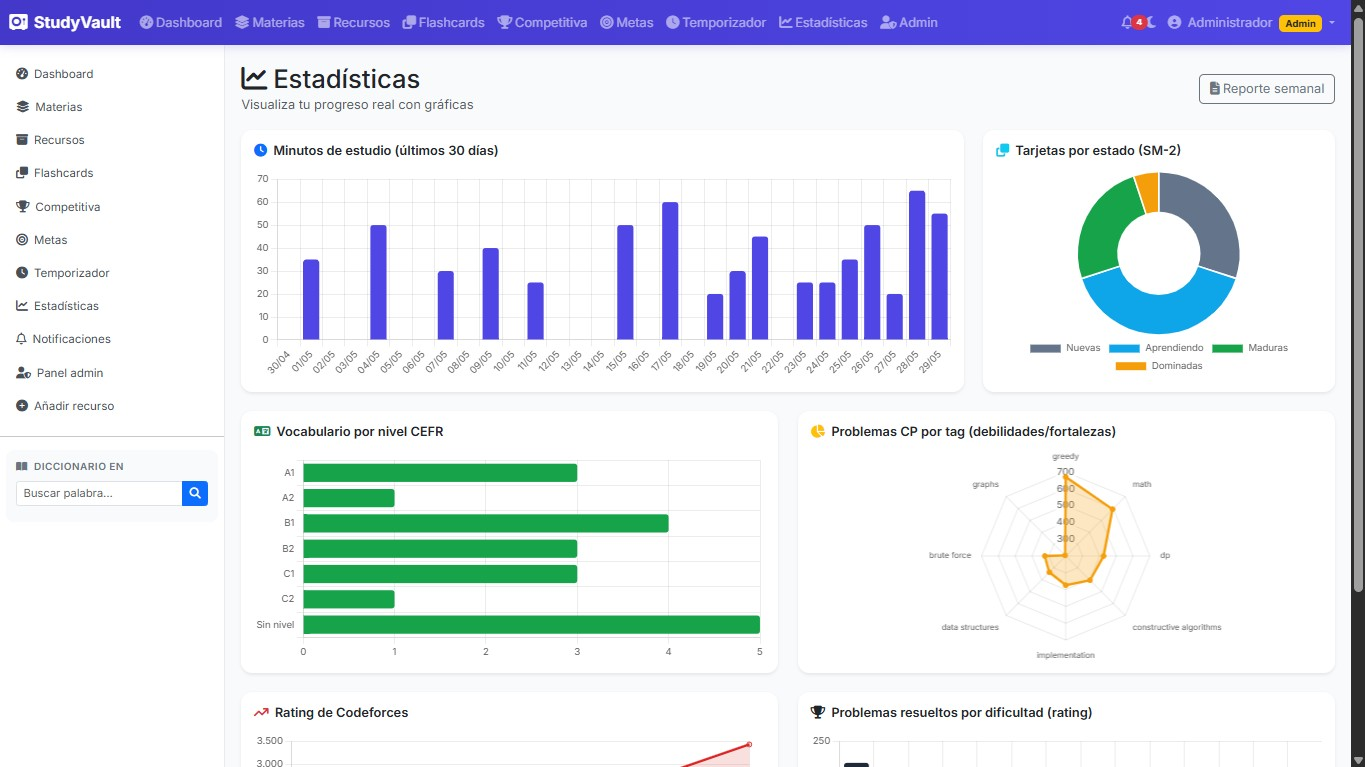
\includegraphics[width=0.95\linewidth]{cap_08_estadisticas.jpg}
    \caption{Panel de Estadísticas con las 6 gráficas Chart.js renderizando datos reales.}
\end{figure}

\subsubsection{Notificaciones -- \cumple}
Centro in-app con badge en navbar, dropdown auto-actualizable y página completa \texttt{?page=notifications}. Generación idempotente por día con 5 reglas: repasos de flashcards, repasos de CP, metas atrasadas, meta diaria sin cubrir, racha en riesgo. Opt-in para Notification API del navegador.

\begin{figure}[H]\centering
    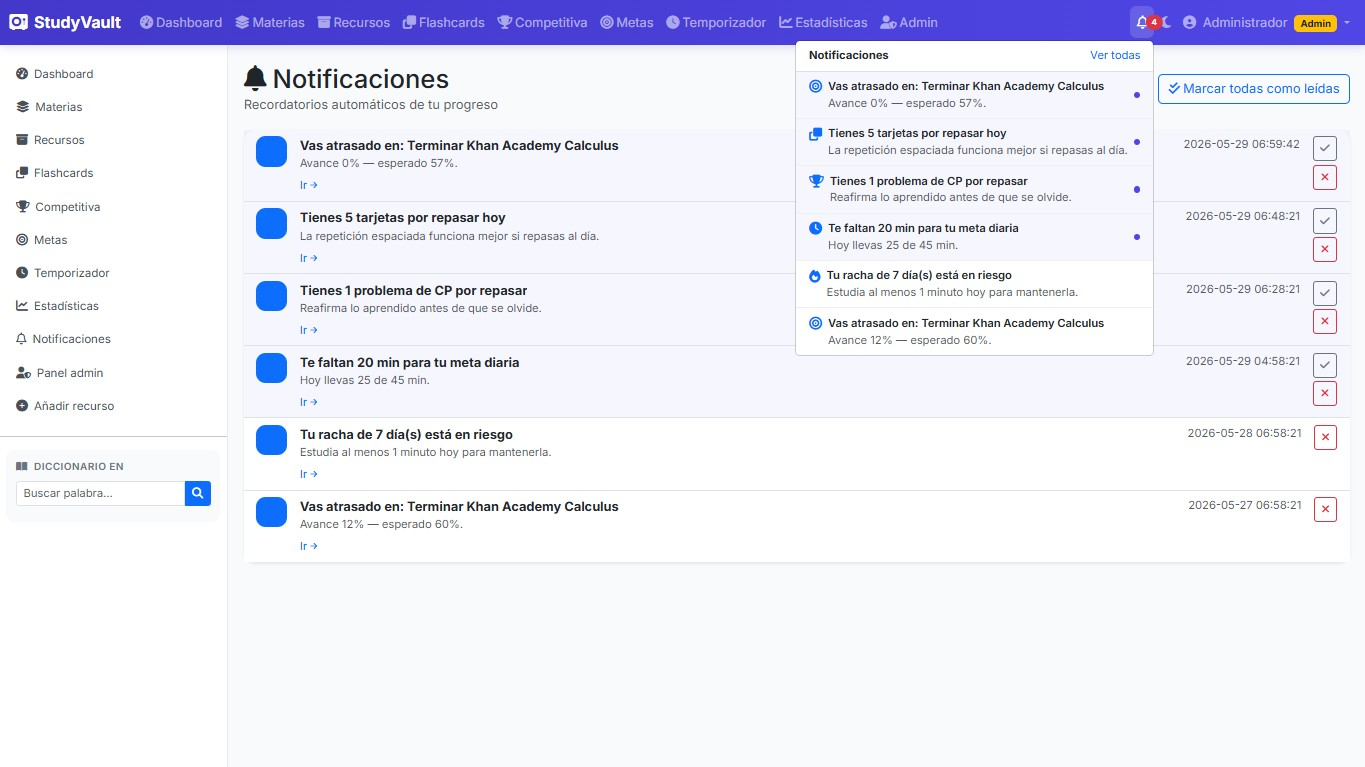
\includegraphics[width=0.95\linewidth]{cap_09_notificaciones.jpg}
    \caption{Centro de notificaciones: campana del navbar con dropdown desplegado mostrando los avisos generados automáticamente.}
\end{figure}

\subsubsection{Tema oscuro -- \cumple}
Toggle persistente en \texttt{localStorage} usando variables CSS bajo \texttt{[data-theme="dark"]}.

\subsubsection{Bitácora de acciones -- \cumple}
Tabla \texttt{activity\_log} + helper \texttt{log\_activity()}.

\subsection{Nivel avanzado (opcionales no requeridos)}

\subsubsection{Panel administrativo -- \parcial}
Implementado un mini-panel con: listado paginado de usuarios con búsqueda, activar / desactivar, 8 tarjetas de totales globales (usuarios, materias, recursos, flashcards, problemas CP, metas, sesiones, minutos). Falta auditoría granular por usuario.

\begin{figure}[H]\centering
    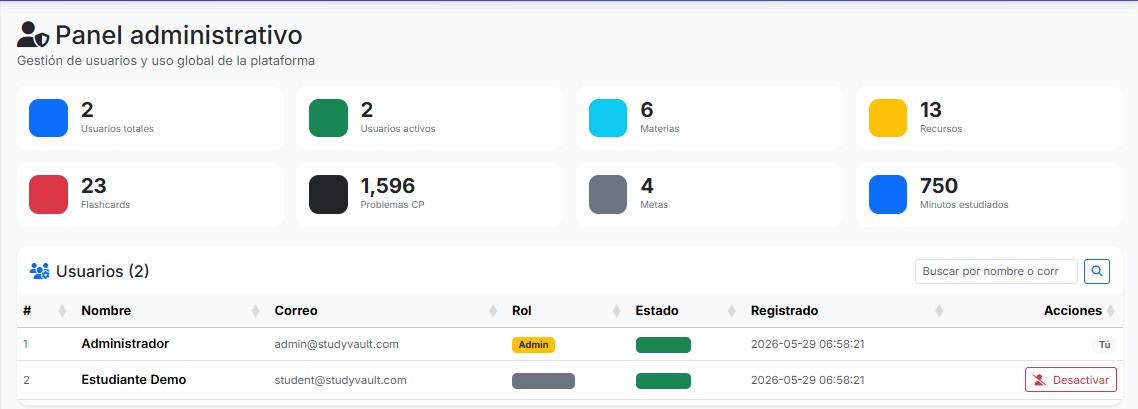
\includegraphics[width=0.95\linewidth]{cap_06_admin.jpg}
    \caption{Panel administrativo: gestión de usuarios con búsqueda + estado activo/inactivo + métricas globales de la plataforma.}
\end{figure}

\subsubsection{API REST propia -- \nocumple}
Existen endpoints JSON internos (\texttt{api/*.php}) pero no una API REST documentada con versiones.

\subsubsection{WebSockets / Chat -- \nocumple}
No aplica al propósito (estudio individual).

\subsubsection{Docker / Framework PHP -- \nocumple}
Mejoras de despliegue/escala, opcionales.

% ---------------------------------------------------------------------
\section{Entregables}

\begin{itemize}[leftmargin=*]
    \item \textbf{Documentación:} \texttt{README.md}, \texttt{MANUAL\_USUARIO.md}, \texttt{DESCRIPCION\_PROYECTO.md}, \texttt{PLAN\_IMPLEMENTACION.md}, \texttt{GUION\_EXPOSICION.md}.
    \item \textbf{Código fuente:} organizado en MVC, comentado.
    \item \textbf{Base de datos:} \texttt{ENTREGA/studyvault\_completo.sql} -- esquema canónico + datos demo en un solo archivo.
    \item \textbf{Manual de usuario:} cubre todas las funciones.
\end{itemize}

% ---------------------------------------------------------------------
\section{Métricas finales del proyecto}

\begin{tabular}{lr}
\toprule
\textbf{Métrica} & \textbf{Valor} \\
\midrule
Tablas en la BD                  & 16 \\
Modelos PHP (OOP)                & 12 \\
Controladores                    & 11 \\
Vistas                           & 26 \\
Proxies de API externa           & 5 \\
APIs externas integradas         & 4 \\
Pruebas automatizadas (assert)   & 53 \\
Gráficas Chart.js                & 6 \\
Migraciones documentadas (v2--v8)& 7 \\
Líneas SQL de esquema canónico   & $\sim$460 \\
\bottomrule
\end{tabular}

\vspace{1cm}
\hrule
\vspace{0.3cm}
\textit{Documento generado para la entrega final del proyecto de Programación Web.}

\end{document}
